\chapter{Introduction}
\label{ch:introduction}

\newpar
From plain text, the task of extracting semantic relations between two or more entities, is known as Relation Extraction (RE). These relations can exist in different types. For example, \txti{"Germany is in Europe"} states a \txti{"is in"} relationship between \txti{"Germany"} and \txti{"Europe"}. With this information, a triple can be formed, \txti{<Germany, is in, Europe>}. Efficient RE is useful for applications like Knowledge Graph (KG) completion and question answering, which are in turn responsible for dependent applications. 


%%%%%add references %%%%%%%%%%
\newpar
Traditionally, supervised RE techniques produce elevated performance for RE\cite{bibid}. They solely rely on labeled data that is manually annotated. Manual annotation is time consuming and need an army of annotators. It is generally annotated into entities and relationships(entities: \txti{"Germany", "Europe"} relationship: \txti{"is in"}). This limitations strongly suggest need for semi-supervised or unsupervised RE techniques that are reliable enough and can mimic manual annotation.  

\newpar
Distant Supervision (DS) aims at solving this limitation by automatic production of labeled data by aligning KGs and plain text. In this process, it makes an assumption that, if there exists a relationship between two entities (\txti{e1, e2}) in Knowledge Base (KB), then all the sentences that consist \txti{e1, e2} express that relationship in some way\cite{zeng2015distant}. 
In the Fig.\ref{fig:dsexm}, if there exists, a triplet <\txti{John Doe, FounderOf, John Doe Inc.}> then, all the sentences in the plain text that contain \txti{John Doe} and \txti{John Doe Inc.} are considered as the training instances of \txti{FounderOf} relation. From the Table\ref{tab:johndoe}, if the following sentences are considered, DS cannot have better performance as it categorizes relations like, \txti{Recalled}, \txti{ResignedFrom} into \txti{CreatorOf}, \txti{FounderOf} relations respectively. This introduces noise problem. It can be countered using Deep Neural Network (DNN) models, which try to provide a significant improvement, but fail in making predictions due to lack of sufficient background information associated with entities and relationships. For example, from Fig.\ref{fig:dsexm}, there are two sentences generated using DS, they both use \txti{"create"} relation but corresponding relations do not match. They in fact, represent \txti{FounderOf} and \txti{AuthorOf} relations respectively.

\begin{figure}[h!]
	\centering
	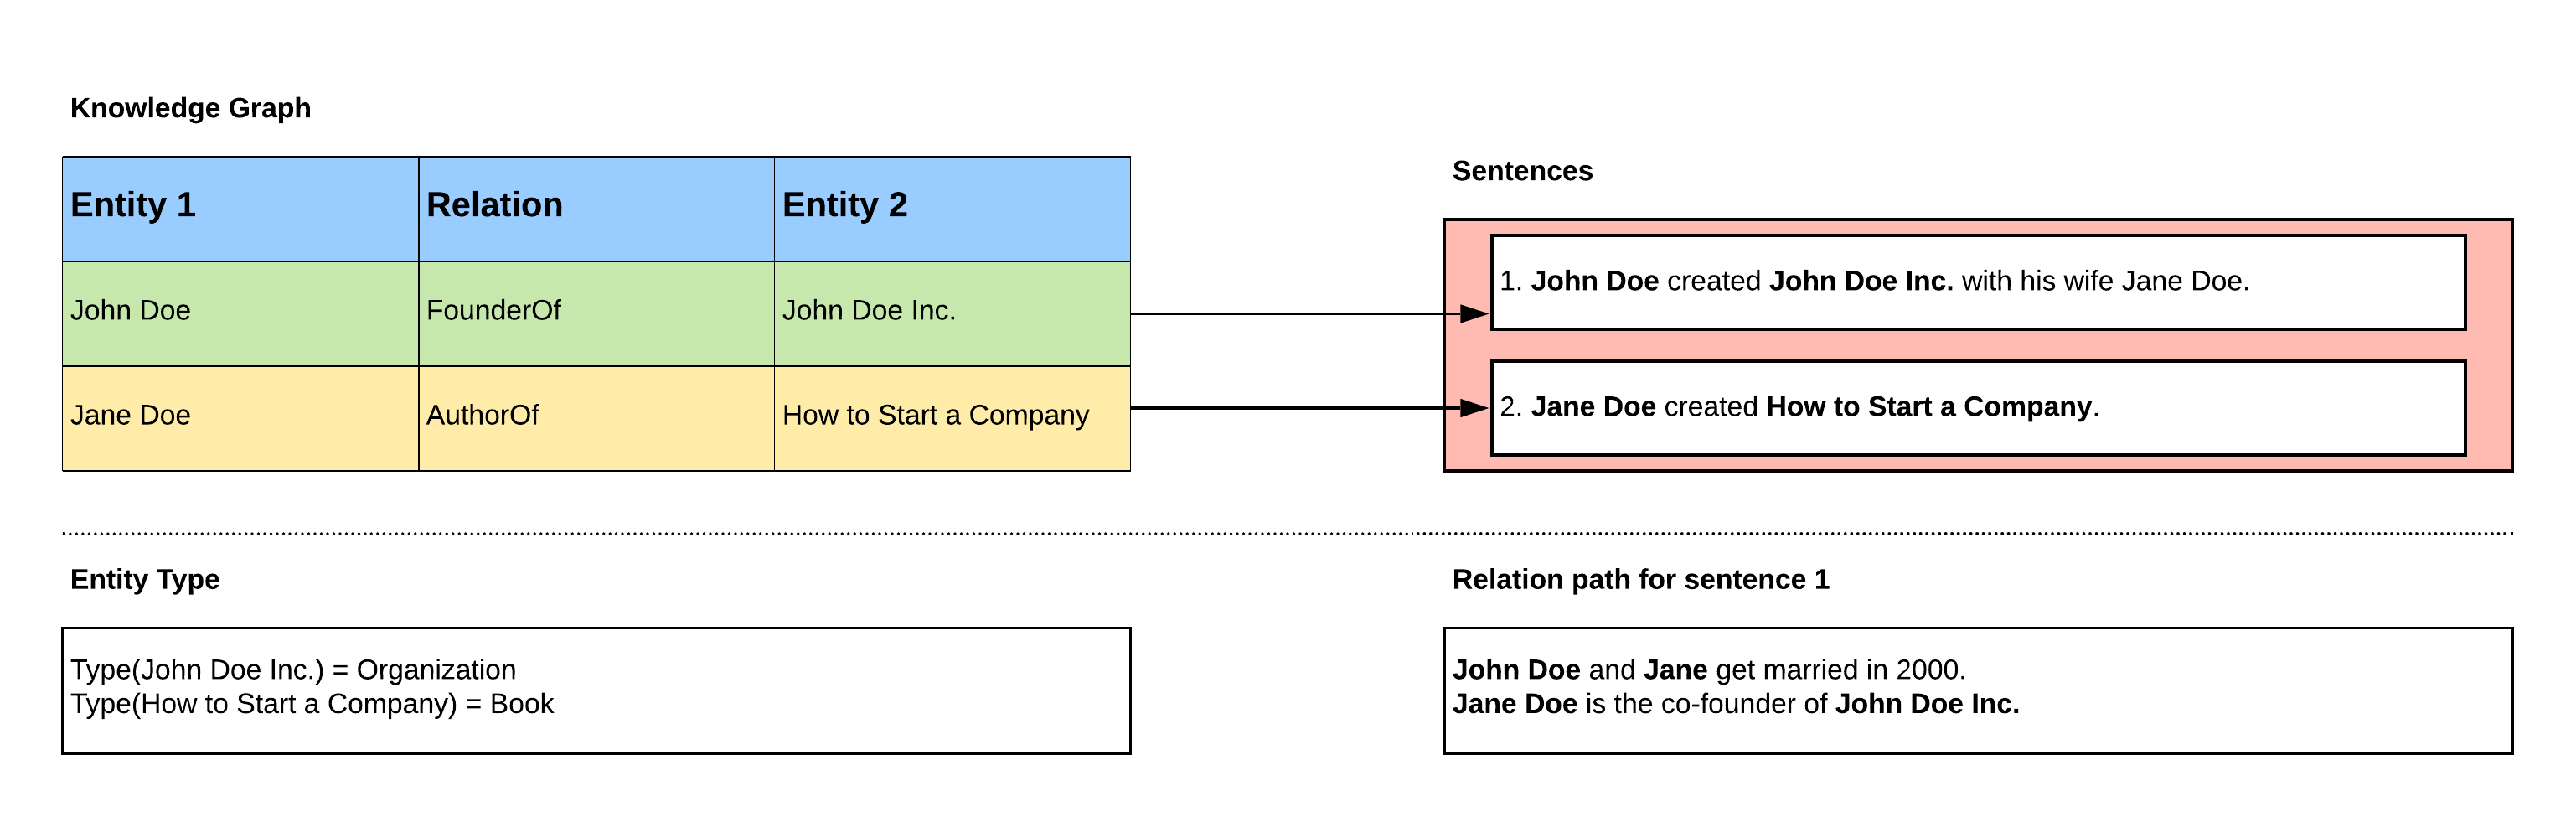
\includegraphics[scale=0.15]{figures/dsexample.PNG}
	\caption{DS Example 1}
	\label{fig:dsexm}
\end{figure}

\begin{table}[]
	\centering
	\begin{tabular}{lllll}
		
		Entity 1 & Relation     & Entity 2      &  &  \\
		John Doe & FounderOf    & John Doe Inc. &  &  \\
		John Doe & CreatorOf    & Doe Glasses.  &  &  \\
		John Doe & Recalled     & Doe Glasses.  &  &  \\
		John Doe & ResignedFrom & John Doe Inc. &  & 
	\end{tabular}
	\caption{DS Example 2}
	\label{tab:johndoe}
\end{table}

%%%%%%%%%%find citations%%%%%%%%%%
DNNs create bias at each stage and especially with long-tail relations, background information tend to be unusable for making predictions. They are mostly constructed for customized models to join knowledge that is limited to incorporate heterogeneous background information in parallel. Some of the methods did not handle the side effect caused due to introduced noise. 

%%%%%%%%introduce the topic%%%%%%%%%%
Graph-based model for DSRE was proposed by Duan et al.\cite{duan2019hybrid} to solve the problems by DSRE. It fuses heterogeneous background information, as well, reduces side effects due to brought in noisy data. Typical process for neural networks start with conversion of different types data into vectors using various types of encoders and store each information in a graph node. Related nodes of graph are combined using a Graph Convolution Network(GCN). This model eases the incorporation of missing data and incorporate it with other graph nodes. Attention mechanism for the graph reduces the introduced noise problem by assigning higher weight for known true information. 